% !TEX root = MAIN.tex
\clearpage
\section{Evaluation of Code-driven Mutation Testing Toolsets}
\label{sec:toolsComparison}

This section describes a preliminary evaluation conducted to identify mutation testing tools that are applicable in space context, based on the case study systems of the project. More precisely, for this preliminary evaluation we considered the case study system provided by LuxSpace.

To carry out this preliminary evaluation of mutation testing tools, we selected from the list of mutation testing tools provided in Table 1.1 of deliverable D1, a subset of tools based on the following criteria:

\begin{itemize}
	\item \textbf{Availability of source code.} To enable optimizations, the tool under analysis should be provided along with source code.
	\item \textbf{Applicability to C/C++ code.} The tool under analysis should be able to process C and C++ code.
	\item \textbf{Licence compatible with ESA Software Community Licence Permissive (ESA SCLP).} The licence of the tool under analysis, should enable redistributing the tool itself within the FAQAS framework, which is released under ESA SCLP.
	\item \textbf{Age.} To avoid problems due to support for recent libraries, we should prioritize tools that are recent and actively developed.
\end{itemize}

% !TEX root =  ../MAIN.tex


\setlength\LTleft{0pt}
\setlength\LTright{0pt}
\scriptsize 
\begin{longtable}{@{\extracolsep{\fill}}|p{3.4cm}|p{2.7cm}|p{7cm}|@{}}
\caption{\normalsize Summary of Data-Driven Mutation Testing Benchmarks.}
\label{table:mutationtools} \\
\hline
\textbf{Reference}                   & \textbf{Approach/Tool Name}      & \textbf{Evaluation} \\
\hline
Hariri \& Shi 2018          & SRCIRor                 &
\begin{minipage}[t]{6.5cm}
\textbf{Source code availability.} Yes, https://github.com/TestingResearchIllinois/srciror.\\
\textbf{Applicability to C/C++ code.} Yes.\\
\textbf{ESA SCLP Compatible.} Yes, released under NCSA, https://opensource.org/licenses/NCSA, which allows redistribution and relicensing.\\
\textbf{Age.} Aged, last update in September 2018.\\
\textbf{Outcome. The tool is applicable in space context.} 
\end{minipage}\\
\hline
Wang et al. 2017            & Accmut                  &
\begin{minipage}[t]{6.5cm}
\textbf{Source code availability.} Yes, https://github.com/wangbo15/accmut/\\
\textbf{Applicability to C/C++ code.} Yes.\\
\textbf{ESA SCLP Compatible.} Yes, released under NCSA, https://opensource.org/licenses/NCSA, which allows redistribution and relicensing.\\
\textbf{Age.} Aged, last update in January 2018.\\
\textbf{Outcome. Depends on CLANG/LLVM, which prevents compilations for some sysems.} 
\end{minipage}\\
\hline
Phan et al. 2018            & MUSIC                   &
\begin{minipage}[t]{6.5cm}
\textbf{Source code availability.} Yes, https://github.com/swtv-kaist/MUSIC/\\
\textbf{Applicability to C/C++ code.} Yes.\\
\textbf{ESA SCLP Compatible.} No. The software is licensed with proprietary licence. In private communication via e-mail, authors have shown to be available to relicensing, however this might not fit the budget of the project.\\
\textbf{Age.} Recent, last update in July 2019.\\
\end{minipage}\\
\hline
Denisov \& Pankevich 2018   & Mull                    &
\begin{minipage}[t]{6.5cm}
\textbf{Source code availability.} Yes, https://github.com/mull-project/Mull\\
\textbf{Applicability to C/C++ code.} Yes.\\
\textbf{ESA SCLP Compatible.} Yes. Apache Licence 2.0, https://opensource.org/licenses/Apache-2.0.\\
\textbf{Age.} Ongoing, last update in June 2020.\\
\textbf{Outcome. The tool requires compilation with CLANG/LLVM, which leads to compilation errors with systems depending on RTEMS. Also, natively, Mull performs mutations on the fly through just-in-time compilation features, which is inapplicable if the SUT is executed within a simulator.} 
\end{minipage}\\
\hline
Delgado et al. 2018         & MuCPP                   &
\begin{minipage}[t]{6.5cm}
\textbf{Source code availability.} No, only executables are available https://ucase.uca.es/mucpp/\\
\end{minipage}\\
\hline
Jia \& Harman 2008          & Milu                    &
\begin{minipage}[t]{6.5cm}
\textbf{Source code availability.} Yes, https://github.com/yuejia/Milu/\\
\textbf{Applicability to C/C++ code.} Yes.\\
\textbf{ESA SCLP Compatible.} Yes, released under NCSA licence, https://opensource.org/licenses/NCSA.\\
\textbf{Age.} Aged, last update in April 2018.\\
\textbf{Outcome. The tool generates a preprocessed source code that does not compile.} 
\end{minipage}\\
\hline
Brannstrom et al. 2015      & Dextool                 &
\begin{minipage}[t]{6.5cm}
\textbf{Source code availability.} Yes, https://github.com/joakim- brannstrom/dextool\\
\textbf{Applicability to C/C++ code.} Yes.\\
\textbf{ESA SCLP Compatible.} Yes, released under Mozilla public Licence 2.0, https://opensource.org/licenses/MPL-2.0.\\
\textbf{Age.} Ongoing, last update in June 2020.\\
\textbf{Outcome. Depends on CLANG/LLVM, which prevents compilations for some sysems.} 
\end{minipage}\\
\hline
Delamaro et al. 2001        & Proteum                 &
\begin{minipage}[t]{6.5cm}
\textbf{Source code availability.} Yes, https://github.com/magsilva/proteum.\\
\textbf{Applicability to C/C++ code.} Yes.\\
\textbf{Age.} Aged, last update December 2015.\\
\end{minipage}\\
\hline
Shariar and Zulkernine 2008 & Function Calls Mutation &
\begin{minipage}[t]{6.5cm}
\textbf{Source code availability.} No.\\
\end{minipage}\\
\hline
Dans \& Hierons 2001        & Floating-point Mutation &
\begin{minipage}[t]{6.5cm}
\textbf{Source code availability.} No.\\
\end{minipage}\\  

\hline                                                           
\end{longtable}


\normalsize


The first three criteria mentioned above constitute mandatory requirements. 
Tools not meeting these requirements are not selected for evaluation in our context because they cannot be integrated into the FAQAS framework.
Table~\ref{table:mutationtools} provides the list of tools appearing in Table~1.1 of deliverable D1 along with the evaluation based on the criteria specified above. We do not evaluate all the criteria when one of the mandatory requirements is not met.
For what it concerns the compatibility with the ESA Software Community Licence Permissive, we consider the licenses NCSA and Apache Licence 2.0 compatible. 
Indeed, both the two licences allow for redistribution of the software, a condition that is sufficient to release a mutation testing tool as component of the FAQAS framework.

For our preliminary evaluation we selected the five most recent tools that fulfill our mandatory requirements: SRCIRor, Mull, Dextool, Accmut, and Milu. Proteum has been discarded because its latest stable version dates back to December 2015; on May 2020 a few changes had been made on Proteum GitHub repository, however, the up to date version is indicated by its developer as not usable.

Section~\ref{subsec:experiment_design} provides an overview of the experiment design and the case study considered. 
Section~\ref{subsec:background} provides a brief introduction to the static analysis framework used by all the tools assessed in our study.
Section~\ref{subsec:srciror} to Section~\ref{subsec:dextool} describe the results achieved for each mutation testing tool considered in our study.

As detailed in the following Sections, the only mutation testing tool that is applicable to space software is SRCIRor.

\subsection{Experiment Design and Case Studies}
\label{subsec:experiment_design}




To evaluate the applicability of existing mutation testing tools to space software, we evaluated each mutation testing tool considered in our study against the same case study system of the project, i.e., the System Test Suite for ESAIL provided by LXS. We selected this case study system, because, based on inspection of its specification documents and source code, appears to be the most complicate to process by mutation testing tools. This is mostly due to three criticalities:

\begin{itemize}
	\item ESAIL is the largest case study system of FAQAS in terms of lines of code;
	\item the ESAIL system test suite requires that the full software is compiled and all the required libraries linked (this may complicate the use of tools that cannot parse all the source code);
	\item the software under test (SUT) is executed within a system emulator (SVF) that requires the SUT to respect its real-time constraints.
\end{itemize}

In the following, we provide an overview of ESAIL and the ESAIL System Test Suite. ESAIL consists of 924 source files (719 files with extension ``.c'' and 205 with extension ``.h''). In total, it consists of 74,161 LOC. ESAIL is compiled with sparc-rtems4.8-gcc, a tailored version of the gcc compiler for sparc systems, the compiler is provided by Cobham Gaisler\footnote{https://www.gaisler.com/index.php/products/operating-systems/rtems}.

\begin{figure}[h]
	\centering
    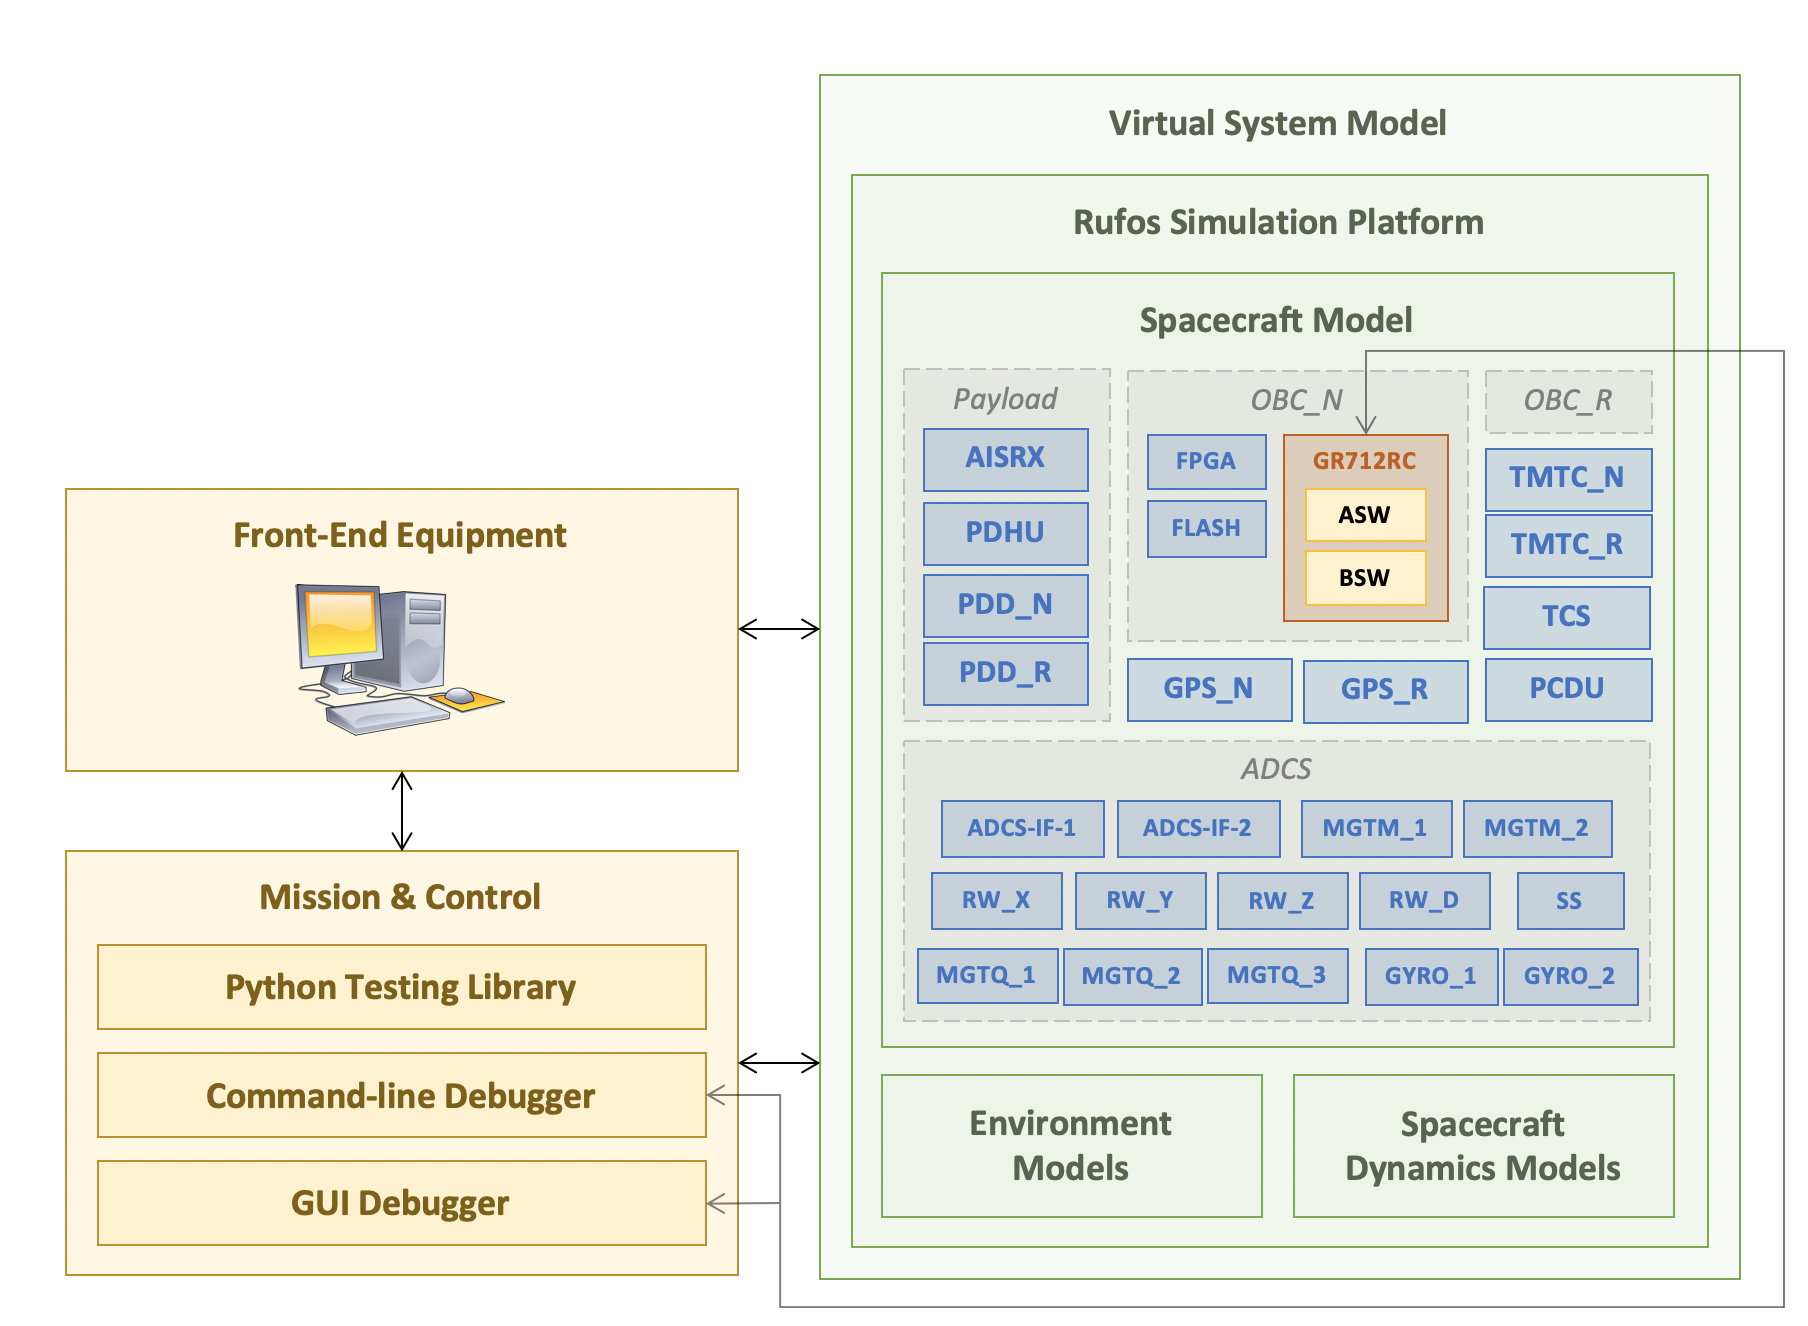
\includegraphics[width=0.7\textwidth]{images/esail}
    \caption{ESAIL system testing environment.}
    \label{fig:esail}
\end{figure}

The architecture of the ESAIL System Testing environment is shown in Figure \ref{fig:esail}. The python testing library is used to execute system test cases that send commands to ESAIL. ESAIL is executed in a simulator based on Rufos. The ESAIL system test suite consists of 121 python programs and it executes in 10 hours, depending on the running environment.

The objective of this preliminary evaluation is to determine if the mutation testing tools considered in our study can process the case study system and automatically generate mutated versions of the case study system that can be successfully compiled and tested. More precisely, we aim to verify if the mutation testing tools considered in our study can successfully create mutated version of ESAIL that can be compiled and executed within the SVF.

\subsection{Background on Clang/LLVM}
\label{subsec:background}

In this section we provide background information on the components that are used by most of the tools considered in our evaluation, i.e., Clang/LLVM.


\begin{figure}[h]
	\centering
    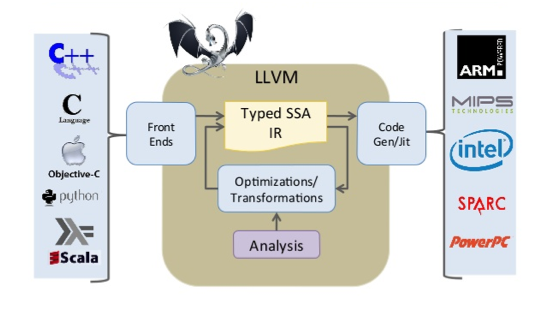
\includegraphics[width=0.5\textwidth]{images/llvm}
    \caption{LLVM compiler infrastructure.}
    \label{fig:llvm}
\end{figure}

The LLVM project is a set of compiler and toolchain technologies. LLVM is designed around an intermediate representation (i.e., LLVM IR) that serves as a portable, high-level assembly language useful for code optimizations. LLVM was originally implemented for C and C++, but now currently it also supports Ada, D, Delphi, Fortran, Haskell, Julia, Objective-C, Rust and Swift. It can be used for performing static analysis on code (e.g., uninitialized memory uses), optimization or code parsing.

Clang is a front-end for LLVM that processes C-family languages: C, C++, Objective C, Objective C++. Clang converts C/C++ to LLVM IR, LLVM performs optimizations on the IR, and the LLVM x86 backend writes out x86 machine code for execution.

\subsection{Evaluation of SRCIRor}
\label{subsec:srciror}

\subsubsection{Overview of the mutation testing tool}

SRCIRor is LLVM-based mutation testing tool that works at the level of source code (SRC), and the LLVM compiler intermediate representation (IR). 
At a source code level SRCIRor performs mutations by using the clang compiler to parse the input files and build the abstract syntax trees (AST). 
At the IR level SRCIRor finds and directly mutates the instructions of interest, which might be all the instructions of the SUT or a subset of them. 
SRCIRor implements six types of operators, it implements Arithmetic Operators (e.g., $+, -, *, /, \%$), Relational Operators (e.g., $<, <=, >, >=, ==, !=$), Logical Operators (e.g., $\&\&, ||$), Bitwise Operators (e.g., $\&, |, \wedge$), Arithmetic Assignment Operators (e.g., $+=, -=, *=, /=, \%=$) and Bitwise Assignment Operators (e.g., $\&=, |=, \wedge=$).

\begin{figure}[h]
	\centering
    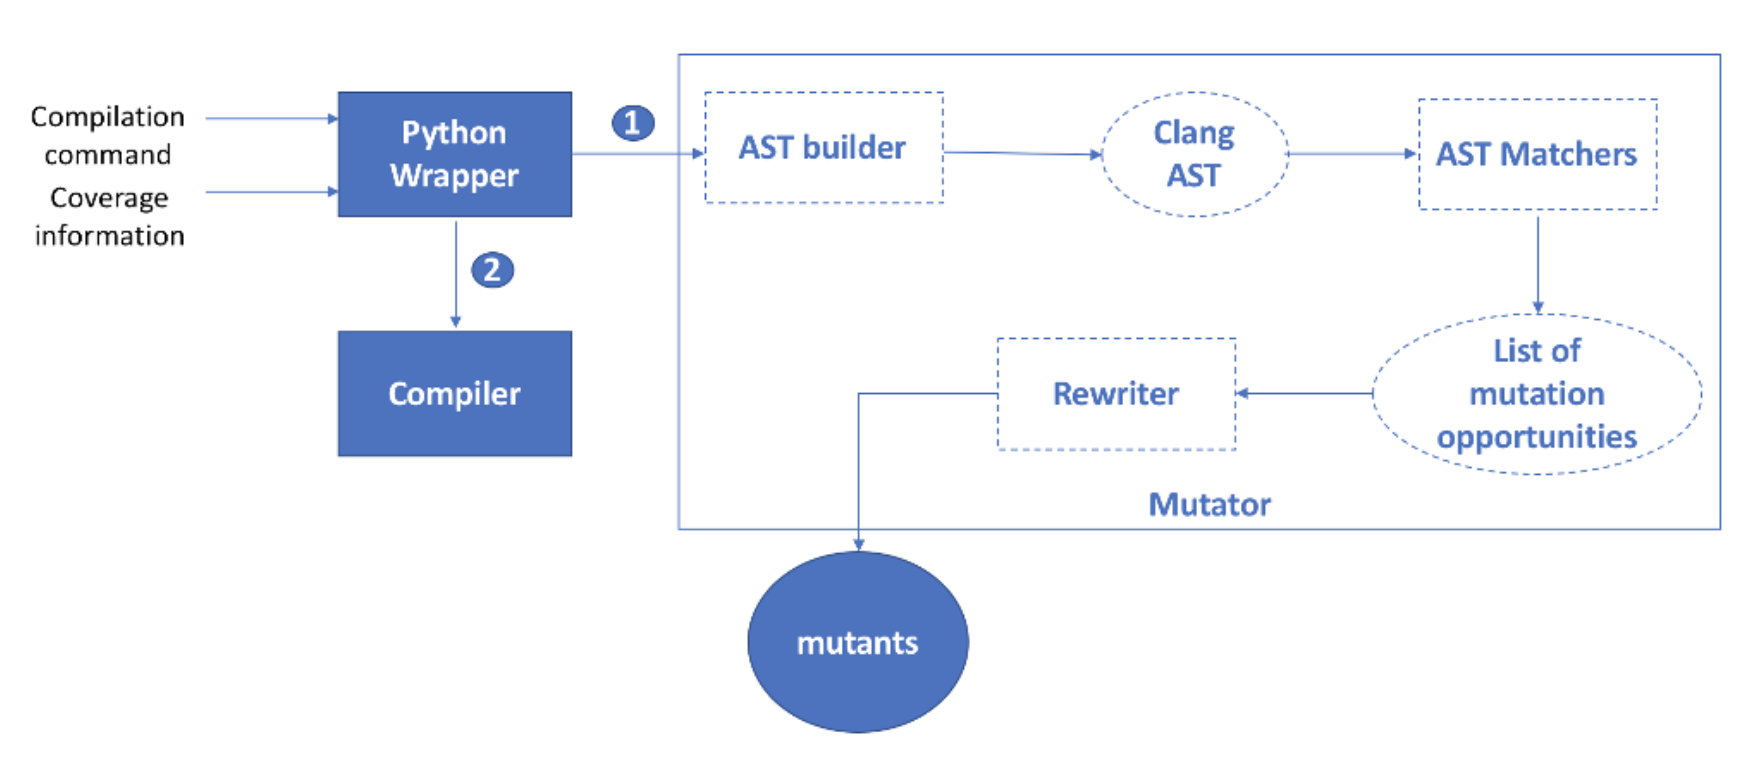
\includegraphics[width=0.75\textwidth]{images/srciror_arch}
    \caption{SRCIRor architecture. Source Hariri et al.~\cite{hariri2018srciror}.}
    \label{fig:srciror_arch}
\end{figure}

\MREVISION{C-P-23}{Figure~\ref{fig:srciror_arch} shows the architecture of SRCIRor. The mutations are done in three steps: in (1) the clang parser with the help of a Python wrapper, processes the input files and builds the abstract syntax tree (AST). Then, in (2), SRCIRor implements ASTMatchers to identify the mutation points along the AST. ASTMatchers are a domain specific language for querying the AST in a simple manner, for example, to implement the ICR mutation operator is enough to make a call to the ASTMatcher \texttt{integerLiteral()} to obtain all the integer literals present in the AST. Finally, in (3), SRCIRor uses again clang to perform the source to source transformation by directly modifying the source code, the transformation is then applied iteratively for all the mutation points identified in (2).}

\subsubsection{Results}

%The main objective of FAQAS of this project is being able to apply mutation testing techniques to space software. To assess the compatibility of SRCIRor with FAQAS we applied the tool to one of our case studies, in this case, we selected the ESAIL SVF software.
The mutation process has been executed by applying the SRCIRor source code mutator to every .c file in the ESAIL SVF project. We applied the default configuration of SRCIRor, that is, applying the six operators and mutating every line within the source code files.
From the results, we observe the generation of 105\,543 mutants. However, during the pass of SRCIRor we detected 1\,060 warnings thrown by the clang input parser.

Most of the warnings are caused by SRCIRor trying to mutate memory addresses declared in C code, (e.g., mutating \texttt{0x03A6} into \texttt{(- 1)x03A6}), and unsigned integer literals (e.g., \texttt{0u}, \texttt{1u} into \texttt{(-1)u}, \texttt{1u}).
Listing~\ref{srciror_1} to Listing~\ref{srciror_10} list the representative cases for all the warning classes found during the mutation process. 

Listing~\ref{srciror_1} shows a warning due to an incompatibility with duplicate keywords declaration. 
Listing~\ref{srciror_2} shows a warning related to the magnitude of a floating-point variable. 
Listing~\ref{srciror_3} shows a warning due to an implicit conversion from an enumeration type. 
Listing~\ref{srciror_4} shows a warning related to an uninitialized variable being used. 
Listing~\ref{srciror_5} shows a warning due to a variable not being used in the source code. 
Listing~\ref{srciror_6} shows a warning related to an invalid cast. 
Listing~\ref{srciror_7} shows a warning related to a clang problem with inline functions. 
Listing~\ref{srciror_8} shows multiple warnings on inline functions and invalid casts.
Listing~\ref{srciror_9} shows a warning due to an inappropriate use of parentheses. Finally, Listing~\ref{srciror_10} shows a warning related to incompatible declarations of already existing library functions. 

% !TEX root = ../MAIN.tex

\noindent\begin{minipage}{\textwidth}
\begin{lstlisting}[language={}, caption=1st warning example., label=srciror_1]
In file included from /home/svf/Obsw/Source/ApplicationLayer/SYS_KeepAlive/Source/SoftKeepAliveTask.c:50: 
././HighLevelDriverLayer/EPS_Handler/Public/epshdl_Api.h:125:104: 
warning: duplicate 'const' declaration specifier [-Wduplicate-decl-specifier]
epshdlr_status_code_t epshdl_MemoryWrite(const uint16_t memAddr, const uint16_t memLen, const uint16_t const *memDataPtr);
													  ^
1 warning generated.
\end{lstlisting}
\end{minipage}
% !TEX root = ../MAIN.tex

\noindent\begin{minipage}{\textwidth}
\begin{lstlisting}[language={}, caption=2nd warning example., label=srciror_2]
/home/svf/Obsw/Source/ApplicationLayer/AdcsController/Source/strtod.c:122:12: warning: magnitude of floating-point constant too large for type 'double'; maximum is 1.7976931348623157E+308 [-Wliteral-range]
return HUGE_VAL; 
			 ^
./_Ext/mlfs/include/mlfs.h:147:19: note: expanded from macro 'HUGE_VAL' #define HUGE_VAL (1.0e999999999)
							^ 
1 warning generated.
\end{lstlisting}
\end{minipage}
% !TEX root = ../MAIN.tex

\noindent\begin{minipage}{\textwidth}
\begin{lstlisting}[language={}, caption=3rd warning example., label=srciror_3]
/home/svf/Obsw/Source/ApplicationLayer/AdcsController/Source/adcs_DetermineSatellitePosition.c: 222:41: warning: implicit conversion from enumeration type 'cast_Status_t' (aka 'enum cast_Status_e') to different enumeration type 'prep_ResponseCode_t' (aka 'enumprep_ResponseCode_e') 
[-Wenum-conversion]
adem_SetDeterminedSatellitePosition(Status,*SatState_Ptr,OnBoardTime);
~~~~~~~~~~~~~~~~~~~~~~~~~~~~~~~~~~~ ^~~~~~ 
1 warning generated
\end{lstlisting}
\end{minipage}
% !TEX root = ../MAIN.tex

\noindent\begin{minipage}{\textwidth}
\begin{lstlisting}[language={}, caption=4th warning example., label=srciror_4]
In file included from /home/svf/Obsw/Source/ApplicationLayer/PDHU_Handler/Source/PDHU_handler.c:40:
In file included from ././ApplicationLayer/PDHU_Handler/Private/PDHU_handler.h:31:
In file included from ././ApplicationLayer/PDHU_Handler/Public/PDHU_handler_Api.h:34: ././HighLevelDriverLayer/EPS_Handler/Public/epshdl_Api.h:125:104: warning: duplicate 'const' declaration specifier [-Wduplicate-decl-specifier]
epshdlr_status_code_t epshdl_MemoryWrite(const uint16_t memAddr, const uint16_t memLen, const uint16_t const *memDataPtr);
														^
/home/svf/Obsw/Source/ApplicationLayer/PDHU_Handler/Source/PDHU_handler.c:1302:8: warning: variable 'received_size' is used uninitialized whenever 'if' condition is false [-Wsometimes- uninitialized]
	if(is_PDHU_on() == true) 
			^~~~~~~~~~~~~~~~~~~~
/home/svf/Obsw/Source/ApplicationLayer/PDHU_Handler/Source/PDHU_handler.c:1316:8: note: uninitialized use occurs here
	if(received_size != PDHU_EVENT_LOG_SIZE) 
			^~~~~~~~~~~~~
/home/svf/Obsw/Source/ApplicationLayer/PDHU_Handler/Source/PDHU_handler.c:1302:5: note: remove the 'if' if its condition is always true
	if(is_PDHU_on() == true)
			^~~~~~~~~~~~~~~~~~~~~~~~ 
/home/svf/Obsw/Source/ApplicationLayer/PDHU_Handler/Source/PDHU_handler.c:1300:27: note: initialize the variable 'received_size' to silence this warning
	uint32_t received_size; 
											  ^
										  	= 0
2 warnings generated.
\end{lstlisting}
\end{minipage}
% !TEX root = ../MAIN.tex

\noindent\begin{minipage}{\textwidth}
\begin{lstlisting}[language={}, caption=5th warning example., label=srciror_5]
/home/svf/Obsw/Source/ApplicationLayer/AdcsDataExchangeManager/Source/adem_GetReactionwheelMeas InEng.c:44:21: warning: unused variable 'RW_ACCELERATION_COEFF' [-Wunused-const-variable]
static const double RW_ACCELERATION_COEFF 	= 3.75e-3;
/* RW_ACCELERATION_COEFF 0.00375 rpm/s per digit as per ICD RW 90

1 warning generated.
\end{lstlisting}
\end{minipage}
% !TEX root = ../MAIN.tex

\noindent\begin{minipage}{\textwidth}
\begin{lstlisting}[language={}, caption=6th warning example., label=srciror_6]
/home/svf/Obsw/Source/HighLevelDriverLayer/OBC_Handler/Source/ObcHandler_ProcessingTask.c:130:3 6: warning: cast to 'uint8_t *' (aka 'unsigned char *') from smaller integer type 'unsigned int' [-Wint-to-pointer-cast]
	CurrentSampleAddress_ptr = (uint8_t*)(EEPROM_START_ADDRESS + PATTERN_OFFSET + PatternCheck[SampleIndex].Offset);
															^
1 warning generated.
\end{lstlisting}
\end{minipage}
% !TEX root = ../MAIN.tex

\noindent\begin{minipage}{\textwidth}
\begin{lstlisting}[language={}, caption=7th warning example., label=srciror_7]
In file included from /home/svf/Obsw/Source/LowLevelDriverLayer/apbuart/Source/drv_uart.c:47: ././LowLevelDriverLayer/core/Public/coreApi.h:193:12: warning: inline function 'loadmem' is not defined [-Wundefined-inline]
inline int loadmem(int addr); /home/svf/Obsw/Source/LowLevelDriverLayer/apbuart/Source/drv_uart.c:553:18: note: used here
	reg_status = loadmem((int)&uart->regs->status);
In file included from /home/svf/Obsw/Source/LowLevelDriverLayer/apbuart/Source/drv_uart.c:61: ././LowLevelDriverLayer/apbuart/Private/drv_uartFifo.h:100:20: warning: inline function 'ff_FifoIsEmpty' is not defined [-Wundefined-inline]
extern inline bool ff_FifoIsEmpty(uint32_t const Fifo_ID); /home/svf/Obsw/Source/LowLevelDriverLayer/apbuart/Source/drv_uart.c:653:13: note: used here
	if (ff_FifoIsEmpty(uart->txfifoId) == true)
In file included from /home/svf/Obsw/Source/LowLevelDriverLayer/apbuart/Source/drv_uart.c:61: ././LowLevelDriverLayer/apbuart/Private/drv_uartFifo.h:108:24: warning: inline function 'ff_FifoBytesWaiting' is not defined [-Wundefined-inline]
extern inline uint32_t ff_FifoBytesWaiting(uint32_t const Fifo_ID); /home/svf/Obsw/Source/LowLevelDriverLayer/apbuart/Source/drv_uart.c:1047:30: note: used here
	NbBytesWaiting = ff_FifoBytesWaiting(uart->rxfifoId); 

3 warnings generated.
\end{lstlisting}
\end{minipage}
% !TEX root = ../MAIN.tex

\noindent\begin{minipage}{\textwidth}
\begin{lstlisting}[language={}, caption=8th warning example., label=srciror_8]
/home/svf/Obsw/Source/LowLevelDriverLayer/GRTC/Source/drv_GRTC.c:235:15: warning: cast to 'unsigned short *' from smaller integer type 'unsigned int' [-Wint-to-pointer-cast]
	if ((*(unsigned short *)(rp)&0x00ff) == 0x01) 
				 ^
/home/svf/Obsw/Source/LowLevelDriverLayer/GRTC/Source/drv_GRTC.c:244:36: warning: cast to 'unsigned short *' from smaller integer type 'unsigned int' [-Wint-to-pointer-cast]
	cnt = grtcprv_scan((unsigned short *)(rp), upper, 0x01, &found); 
											^			
/home/svf/Obsw/Source/LowLevelDriverLayer/GRTC/Source/drv_GRTC.c:396:46: warning: cast to 'unsigned short *' from smaller integer type 'int' [-Wint-to-pointer-cast]
	if (grtcprv_check_ending((unsigned short *)(rp), cnt - 2, 1)) 
														^
/home/svf/Obsw/Source/LowLevelDriverLayer/GRTC/Source/drv_GRTC.c:404:46: warning: cast to 'unsigned short *' from smaller integer type 'int' [-Wint-to-pointer-cast]
	if (grtcprv_check_ending((unsigned short *)(rp), cnt, 0)) 
														^
/home/svf/Obsw/Source/LowLevelDriverLayer/GRTC/Source/drv_GRTC.c:514:41: warning: 'unsigned short *' from smaller integer type 'unsigned int' [-Wint-to-pointer-cast]
	if ((tot = grtcprv_copy((unsigned short *)(rp), buf, cnt)) != cnt) 
													 ^
In file included from /home/svf/Obsw/Source/LowLevelDriverLayer/GRTC/Source/drv_GRTC.c:50: ././LowLevelDriverLayer/core/Public/coreApi.h:193:12: warning: inline function 'loadmem' is not defined [-Wundefined-inline]
	inline int loadmem(int addr);
							^
/home/svf/Obsw/Source/LowLevelDriverLayer/GRTC/Source/drv_GRTC.c:203:10: note: used here
	rp = loadmem((int)&grtcDev.regs->rrp); 
			 ^

6 warnings generated.
\end{lstlisting}
\end{minipage}
% !TEX root = ../MAIN.tex

\noindent\begin{minipage}{\textwidth}
\begin{lstlisting}[language={}, caption=9th warning example., label=srciror_9]
/home/svf/Obsw/Source/ServiceLayer/Data_Store/Source/Store_TM.c:995:35: warning: equality comparison with extraneous parentheses [-Wparentheses-equality]
	if((Storage_Ptr->tail == Storage_Ptr->header)) 
			~~~~~~~~~~~~~~~~~~^~~~~~~~~~~~~~~~~~~~~~
/home/svf/Obsw/Source/ServiceLayer/Data_Store/Source/Store_TM.c:995:35: note: remove extraneous parentheses around the comparison to silence this warning
	if((Storage_Ptr->tail == Storage_Ptr->header)) 
			~									^			~
/home/svf/Obsw/Source/ServiceLayer/Data_Store/Source/Store_TM.c:995:35: note: use '=' to turn this equality comparison into an assignment
	if((Storage_Ptr->tail == Storage_Ptr->header)) 
												^~
						  					=
1 warning generated.
\end{lstlisting}
\end{minipage}
% !TEX root = ../MAIN.tex

\noindent\begin{minipage}{\textwidth}
\begin{lstlisting}[language={}, caption=10th warning example., label=srciror_10]
In file included from /home/svf/Obsw/Source/Utilities/Misc/Source/mini_rtl.c:31: ././Utilities/Misc/Public/mini_rtl.h:14:10: warning: incompatible redeclaration of library function 'strlen' [-Wincompatible-library-redeclaration]
	unsigned strlen(const char *q);
					  ^
././Utilities/Misc/Public/mini_rtl.h:14:10: note: 'strlen' is a builtin with type 'unsigned long (constchar *)'
././Utilities/Misc/Public/mini_rtl.h:17:5: warning: incompatible redeclaration of library function 'memcmp' [-Wincompatible-library-redeclaration]
	int memcmp(const char *s1, const char *s2, size_t n);
			^
././Utilities/Misc/Public/mini_rtl.h:17:5: note: 'memcmp' is a builtin with type 'int (const void *, const void *, unsigned long)'

2 warnings generated.
\end{lstlisting}
\end{minipage}

To evaluate if the generated mutants can be successfully compiled, we executed the ESAIL compilation process for all the generated 105\,543 mutants. From the total, 103\,747 mutants (98.3\%) were compiled successfully using the original ESAIL settings.

\subsection{Evaluation of Mull}
\label{subsec:mull}

\subsubsection{Overview of the mutation testing tool}

Mull is an open source tool for mutation testing of C/C++ software based on the LLVM framework. Mull works at the intermediate representation level, i.e., the mutations are applied on the instructions residing in the LLVM bitcode files. It relies on debug information to show results, for this reason it requires that the SUT is compiled with clang and the \texttt{-fembed-bitcode} and debug information enabled. \MREVISION{C-P-25}{Mull does not work at source code level.}

The mutation process in Mull consists of the following steps: (1) extracting bitcode files from the executable artifact, (2) finding test cases related to the executable by running the test suite, (3) searching/filtering for mutation points, based on the coverage of the test suite execution, (4) compiling the possible mutations, (5) inserting memory trampolines on the original functions, then compile only the part of bitcode that had been mutated, and (6) running the test cases that cover the mutated function.

Mull generates mutants on the fly, while the SUT is executed against the test suite. To this end it relies on the JIT feature of LLVM. This feature enables the compilation of code on the fly as it is needed, with no necessity of re-compiling the whole program on disk. The online nature of Mull enables it to implement a set of optimizations that speed up the mutation process. A list of optimizations follows.

\begin{itemize}
	\item Dynamic Call Tree: optimization for mutating source code reachable by the test cases
	\item LLVM JIT engine: compilation and linking of the new mutants happen in memory, thus there is no disk I/O overhead.
	\item Sandboxing: run each test in a separate child process, this way, if the child process fails it will not affect the parent process.
	\item Dry-run: collect information in advance about how many mutations a project has and how much time does it take to run it.
	\item Caching: save mutants on disk; for future executions Mull tries first loading the object file from the cache first.
	\item Fail-fast mode: once a mutant is killed by a test case it is no longer executed against other test cases.
\end{itemize}

Although the optimization features of Mull reduce the overall execution time of the mutation process, the online nature of Mull prevents its application to ESAIL. Indeed, ESAIL runs within an emulated environment that requires an executable compiled for the actual platform of the system. This prevents the execution of the JIT feature of the LLVM infrastructure. In the following paragraphs, we provide an overview of the modifications we implemented on Mull to apply it to our case study.

\subsubsection{Extending Mull's features}

%To evaluate Mull, we mutated one of the example projects provided by the tool authors, the fmt library. The fmt library is an open-source formatting library for C++\footnote{https://github.com/fmtlib/fmt} that can be used as alternative to (s)printf and iostreams.

We adapted Mull to statically generate mutants and save them permanently. Specifically, we developed a module that generates an object file each time a new mutant is identified for a specific module. Then, to generate the final executable, we perform the following actions for each mutated object file: (1) replace the original object file with the mutated one, (2) re-launch the original Makefile (this will generate a new version of the program), and (3) save the executable with a specific identifier (i.e., program name followed by the identifier of the mutant created by Mull).

\subsubsection{Results}

Mull requires compilation with clang. For this reason, we had to replace the original \texttt{rtems-gaisler-gcc} compiler with clang. In particular, we compiled ESAIL with four different compilers:

\begin{enumerate}
	\item RTEMS 4.10 and clang 5 (LLVM version)
	\item RTEMS 5 and gcc (RTEMS version)
	\item RTEMS 5 and clang (RTEMS version)
	\item RTEMS 4.8 and clang 9 (LLVM version)
\end{enumerate}

\begin{enumerate}
	\item \textbf{Compilation with RTEMS 4.10 and clang 5 (LLVM version)}

	To successfully compile the project and address "unsupported target" errors we have modified the following in the RTEMS definition files:

	\begin{itemize}
		\item \texttt{/opt/rtems-4.10/sparc-rtems/include/machine/\_types.h}: commented from line 15 to line 29 (error unsupported target)
	\end{itemize}

	However, we did not succeed in compiling the project because clang does not handle the architectures supported by RTEMS. This is shown by the error:

	% !TEX root = ../MAIN.tex

\noindent\begin{minipage}{\textwidth}
\begin{lstlisting}[language={}]
/opt/rtems-4.10/sparc-rtems/leon3/lib/include/sys/ioccom.h:94:9: error: unknown type name 'u_int32_t' typedef u_int32_t ioctl_command_t;
\end{lstlisting}
\end{minipage}

	\item \textbf{Compilation with RTEMS 5 and clang (RTEMS version)}

	To compile the system, we modified the following in the ESAIL source code:

	\begin{itemize}
		\item \texttt{./ApplicationLayer/SystemInit/Public/systemInit.h}: as shown in the example of the source \texttt{rtems-soft-float.c} we set to false the if condition at the line 99. The problem is that several \texttt{drvmgr.h} constant definitions are no longer available in RTEMS 5.
		
		\item \texttt{./LowLevelDriverLayer/apbuart/Source/drv\_uart.c}: commented the inclusion of the header \texttt{\textless rtems/score/types.h\textgreater}, because it does not exist anymore on RTEMS 5.

		\item \texttt{./ProtocolLayer/CANDispatcher/Source/process\_Heartbeat.c}: the constant \texttt{RTEMS\_CLOCK\_GET\_TICKS\_SINCE\_BOOT} is no longer defined in RTEMS 5, so we made the following change:
		
		\begin{itemize}
			\item Modified this line: \texttt{rtems\_clock\_get(RTEMS\_CLOCK\_GET\_TICKS\_SINCE\_BOOT, \&current\_time);}
			\item By this one:        \texttt{current\_time = rtems\_clock\_get\_ticks\_since\_boot();}
		\end{itemize}
		
		\item \texttt{./Utilities/Misc/Source/cpuLoad.c}: the class \texttt{rtems\_tcb} no longer contains a field called \texttt{real\_priority}, in RTEMS now is \texttt{Real\_priority.priority}, so we applied the change.
	\end{itemize}

	In this case, the ESAIL SVF compiles, but with several warnings, an example is shown in Listing~\ref{rtems5_error}.

	% !TEX root = ../MAIN.tex

\noindent\begin{minipage}{\textwidth}
\begin{lstlisting}[language={}, caption=ESAIL compilation warning with RTEMS 5 and clang., label=rtems5_error]
In file included from ./ApplicationLayer/Operational_Sequences/Source/SpacecraftConfigurationVector.c:36: ./Utilities/./Tools/Public/tool_DataManipulationApi.h:174:9: warning: 'BIT_SET' macro redefined [-Wmacro-redefined]
#define BIT_SET(_InputValue,_BitPos) ((_InputValue) |= (1u << (_BitPos)))
	^
/opt/rcc-1.3-rc6-llvm/bin/../sparc-gaisler-rtems5/include/sys/bitset.h:55:9: note: previous definition is here
#define BIT_SET(_s, n, p) \
	^

1 warning generated.
\end{lstlisting}
\end{minipage}

	Despite successful compilation, the execution did not succeed. When trying to boot up the ESAIL SVF software two errors are thrown that makes impossible the execution of any test case:
	\begin{itemize}
		\item Sender: OBC/OBC1/FPGA, message: Watchdog reset \texttt{[0x00000000]}.
		\item Sender: Python, message: message: No OBC powered.
	\end{itemize}

	\item \textbf{Compilation with RTEMS 5 and gcc (RTEMS version)}

	We switched to gcc instead of clang, to determine if the problems were due to the clang or RTEMS version. For this case, we applied the same changes done for case 2.
	Despite the changes above lead to successful compilation of the object code, they did not solve all the compilation problems. Indeed, an ESAIL executable cannot be created because of linking error, the linker claims several undefined references such as:

	% !TEX root = ../MAIN.tex

\noindent\begin{minipage}{\textwidth}
\begin{lstlisting}[language={}]
ld: warning: cannot find entry symbol start; defaulting to 40000000

/opt/rcc-1.3-rc6-gcc/sparc-gaisler-rtems5/leon3/lib/librtemsbsp.a(bspgetworkarea.o): In function `bsp_work_area_initialize’:
/opt/rcc-1.3-rc6-gcc/src/rcc-1.3- rc6/c/src/lib/libbsp/sparc/leon3/../../../../../../bsps/sparc/shared/start/bspgetworkarea.c:32: undefined reference to `rdb_start'
\end{lstlisting}
\end{minipage}

	\item \textbf{Compilation with RTEMS 4.8 and clang 9 (LLVM version)}
	
	In the fourth attempt of ESAIL compilation, we tried to build the software with the token \texttt{release=true} as suggested by LuxSpace. Even though, clang is now able to handle RTEMS libraries, still we get an error that does not allow successful ESAIL compilation:

	% !TEX root = ../MAIN.tex

\noindent\begin{minipage}{\textwidth}
\begin{lstlisting}[language={}]
error: unexpected token in argument list
__asm__ volatile (" lda [%1]1, %0\n" : "=r"(tmp) : "r"(addr));
	^
<inline asm>:1:13: note: instantiated into assembly here lda [%eax]1, %eax
\end{lstlisting}
\end{minipage}

	From Leon documentation, the number after the brackets means a specific Address Space Identifier (ASI), where in this case 1 means forced cache miss. Applied to the specific, clang does not recognize the 1 after the '[\%1]' token.

\end{enumerate}

\MREVISION{C-P-25}{Even though, Mull implement several runtime optimizations, unfortunately for the scope of this project is not possible to consider it, since it forces the use of a specific compiler (i.e., the clang compiler). Therefore, a mutation testing tool that relies on a specific compiler reduces the chances of applying the technique on the context of space software. For example, ESAIL relies on the Sparc RTEMS compiler, so it would out of the scope if we rely on the Mull toolset.}

\subsection{Milu Evaluation Results}
\label{subsec:milu}

\subsubsection{Overview of the mutation testing tool}

Milu is an efficient and flexible C mutation testing tool designed for both first order and higher order mutation testing. Milu is a LLVM-based tool that works at source-code (SRC) level. It performs mutations by using the clang compiler to parse the input files and build the Abstract Syntax Tree (AST) representation of the source code.

The tool implements the following first-order operators:
\begin{itemize}
	\item Absolute Value Insertion (ABS)
	\item Arithmetic Operator Replacement (AOR)
	\item Logical Connector Replacement (LCR)
	\item Relational Operator Replacement (ROR)
	\item Unary Operator Insertion (UOI)
	\item Integer Constant Replacement (CRCR)
	\item Arithmetic Assignment Mutation (OAAA)
	\item Logical Context Negation (OBBN)
	\item Statement Deletion (SSDL)
\end{itemize}

In addition, it also implements the following memory mutation operators:
\begin{itemize}
	\item Replace calloc with malloc (REC2M)
	\item Remove null character assignment statement (RMNA)
	\item Replace calls malloc, calloc, alloca and realloc with null (REDAWN)
	\item Replace size of the requested block with 0 for dynamic memory allocation functions
	(REDAWZ)
	\item Replace the arguments of the sizeof unary operator with the pointer type equivalent if a
	non-pointer type is specified (RESOTPE)
	\item Replace the arguments of the sizeof unary operator with the non-pointer type equivalent
	if a pointer type is specified (REMSOTP)
	\item Remove free statement (RMFS)
	\item Replace malloc with alloca (REM2A)
	\item Replace calloc with alloca (REC2A) 
\end{itemize}


\subsubsection{Results}

Despite Milu has been highly referenced in the literature, it is, nowadays, an outdated tool that is no longer supported by authors.
To generate mutants with Milu it is necessary to pre-process the source files of the system under test with \texttt{gcc -E}, this option will expand all the macros contained in a single source code file.

In our evaluation, the mutation process has been performed by applying the Milu source code mutator to the \texttt{adcs\_ExecuteReactionwheelDesaturation} source file of the \texttt{ApplicationLayer} component, for this example we selected the \linebreak\texttt{adcs\_ExecuteReactionwheelDesaturation} function to be mutated. We applied the default configuration of Milu, that is, applying all the first-order operators to every line in the function under analysis.

However, the mutation process of this source file leads to a segmentation fault in the line \texttt{if(g\_strcmp0(func\_name, tmp\_node -> text) == 0)} of the \linebreak\texttt{milu\_project\_load\_function\_settings} function in Project.c. In particular, when debugging the mutation process with \texttt{gdb}, we observe that there is a variable called \texttt{tmp\_node->text} that contains corrupted data:

\noindent\begin{minipage}{0.8\textwidth}
\begin{lstlisting}[language={}]
$1 = (gchar *) 0xe <Address 0xe out of bounds>
\end{lstlisting}
\end{minipage}

Through a manual inspection of the Milu source code, we found that there are two functions aimed to clean the abstract syntax tree (e.g., fix\_function\_attribute and clean\_ast) that are introducing corrupted data into the AST data structure processed by Milu.
By commenting out these two functions, it was possible to execute the mutation process of the adcs\_ExecuteReactionwheelDesaturation source file. 

Milu produces 35 mutants belonging to the adcs\_ExecuteReactionwheelDesaturation function.
\EMPH{However, it is not possible to compile any of the 35 mutants produced by Milu.} We observe errors during the ESAIL compilation process, in particular there are errors being thrown from the preprocessed area of the mutant. In Listing~\ref{miluerror}, an example of the error obtained during compilation is shown.

\noindent\begin{minipage}{\textwidth}
\begin{lstlisting}[language={}, caption=Error obtained during mutant compilation process in ESAIL., label=miluerror]
In file included from ././ApplicationLayer/AdcsController/Public/Adcs_Api.h:47,
				 from ./ApplicationLayer/AdcsController/Source/adcs_ExecuteReactionwheelDesaturation.c:33:
././ApplicationLayer/Operational_Sequences/Public/opse_Api.h:445: error: expected ‘=’, ‘,’, ‘;’, ‘asm’ or ‘__attribute__’ before ‘PollDapoValue’
In file included from ./ApplicationLayer/AdcsController/Source/adcs_ExecuteReactionwheelDesaturation.c:38:
././ServiceLayer/Data_Health_Management/Public/hema_Api.h:257: error: expected ‘=’, ‘,’, ‘;’, ‘asm’ or ‘__attribute__’ before ‘HealthManager_IsMonitoringEnabled’
In file included from ./ApplicationLayer/AdcsController/Source/adcs_ExecuteReactionwheelDesaturation.c:41:
././HighLevelDriverLayer/GPS_Handler/Public/GPS_handler_Api.h:69: error: expected ‘=’, ‘,’, ‘;’, ‘asm’ or ‘__attribute__’ before ‘GPS_is_next_state_forced’
././HighLevelDriverLayer/GPS_Handler/Public/GPS_handler_Api.h:76: error: expected ‘=’, ‘,’, ‘;’, ‘asm’ or ‘__attribute__’ before ‘GPS_is_state_change_pending
\end{lstlisting}
\end{minipage}

\subsection{Dextool Evaluation Results}
\label{subsec:dextool}

\subsubsection{Overview of the mutation testing tool}

Dextool is a framework for writing plugins using the clang compiler. Mutation testing features are implemented by the Dextool plugin named Mutate, which targets mutation on C/C++ software.

\subsubsection{Results}

Dextool requires the software under test to be compiled with \emph{clang}.
Since the evaluation for Mull has shown that it is not feasible to compile ESAIL with \emph{clang}, we did not perform further experiments with dextool.



\subsection{Accmut Evaluation Results}
\label{subsec:dextool}

\subsubsection{Overview of the mutation testing tool}

Accmut is a mutation testing framework for C programs built on the top of LLVM version 3.8. AccMut generates mutants on LLVM IR level and integrates some optimizations, such as mutation schemata, split-stream execution, and dynamic mutation analysis.

\subsubsection{Results}

Accmut requires the software under test to be compiled with \emph{clang}.
Since the evaluation for Mull has shown that it is not feasible to compile ESAIL with \emph{clang}, we did not perform further experiments with Accmut.


